% ============================================================================
% Lecture 06 (B05): Deep Equilibrium Nets --- The Central Idea
% Deep Learning for Solving and Estimating Dynamic Models in Economics and Finance
% Course author: Simon Scheidegger
% ============================================================================

\documentclass[aspectratio=169,11pt]{beamer}

% ---------- Theme and colors ----------
\usecolortheme{dove}
\setbeamertemplate{navigation symbols}{}
\setbeamertemplate{footline}{%
  \hfill\usebeamerfont{page number in head/foot}%
  \usebeamercolor[fg]{normal text}%
  \insertframenumber\,/\,\inserttotalframenumber\kern1em\vskip4pt}
\setbeamerfont{frametitle}{size=\huge}

% ---------- Packages ----------
\usepackage[utf8]{inputenc}
\usepackage[T1]{fontenc}
\usepackage{amsmath,amssymb,amsfonts}
\usepackage{bm}
\usepackage{graphicx}
\usepackage{tikz}
\usetikzlibrary{shapes,arrows.meta,positioning,calc,fit,backgrounds,patterns,decorations.pathreplacing}
\usepackage{pgfplots}
\pgfplotsset{compat=1.18}
\usepackage{booktabs}
\usepackage{hyperref}
\usepackage{multicol}
\usepackage{xcolor}
\usepackage{algorithm}
\usepackage{algorithmic}

% ---------- Custom colors ----------
\definecolor{uzhblue}{rgb}{0,0,0.5}
\definecolor{uzhgreylight}{RGB}{236,238,241}
\definecolor{uzhgreydark}{RGB}{81,86,94}
\definecolor{harvardcrimson}{RGB}{153,0,0}
\definecolor{unil@blue}{RGB}{0,140,204}
\definecolor{unil@black}{RGB}{35,31,32}
\definecolor{darkgreen}{RGB}{0,100,0}
\definecolor{darkred}{RGB}{139,0,0}
\definecolor{softblue}{RGB}{70,130,180}
\definecolor{softorange}{RGB}{230,159,0}
\definecolor{softgreen}{RGB}{0,158,115}

% ---------- Set beamer colors ----------
\setbeamercolor{frametitle}{bg=uzhgreylight, fg=uzhblue}
\setbeamercolor{title}{fg=uzhblue}
\setbeamercolor{structure}{fg=uzhblue}
\setbeamercolor{block title}{bg=unil@blue, fg=white}
\setbeamercolor{block body}{bg=uzhgreylight}
\setbeamercolor{block title alerted}{bg=darkred,fg=white}
\setbeamercolor{block body alerted}{bg=red!5}
\setbeamercolor{block title example}{bg=darkgreen,fg=white}
\setbeamercolor{block body example}{bg=green!5}
\setbeamercolor{item}{fg=unil@black}
\setbeamercolor{normal text}{fg=unil@black}

% ---------- Emphasis and hyperlinks ----------
\newcommand{\emphc}[1]{\textcolor{harvardcrimson}{#1}}
\hypersetup{colorlinks,linkcolor=harvardcrimson,urlcolor=harvardcrimson}

% ---------- Math commands ----------
\newcommand{\x}{\bm{x}}
\newcommand{\w}{\bm{w}}
\newcommand{\bb}{\bm{b}}
\newcommand{\z}{\bm{z}}
\newcommand{\W}{\bm{W}}
\newcommand{\X}{\bm{X}}
\renewcommand{\a}{\bm{a}}
\newcommand{\R}{\mathbb{R}}
\newcommand{\E}[1]{\mathbb{E}\!\left[#1\right]}
\DeclareMathOperator*{\argmin}{arg\,min}
\DeclareMathOperator*{\argmax}{arg\,max}

% ---------- Title ----------
\title[Lecture 03 (B02)]{Lecture 03 (B02): Deep Equilibrium Nets}
\subtitle{From representative-agent Brock--Mirman through stochastic models, KKT constraints, and loss kernels}
\author{Simon Scheidegger}
\institute{HEC, University of Lausanne}
\date{}
\begin{document}

% Custom command used in some "Finger Exercise" frame titles.
\providecommand{\exercisepause}{%
  \tikz[baseline=(X.base)]{\node[fill=darkgreen!80!black, text=white,
  rounded corners=2pt, inner sep=3pt, font=\scriptsize\bfseries](X){PAUSE};}}

{\setbeamercolor{background canvas}{bg=uzhgreylight}
\begin{frame}
\titlepage
\end{frame}
}

% --- About-this-lecture orientation ---

\begin{frame}{Outline}
\begin{enumerate}
    \item \textbf{Motivation}\\
    {\small Why heterogeneous-agent models? The curse of dimensionality.}

    \vspace{0.4em}
    \item \textbf{From ANNs to Deep Equilibrium Nets}\\
    {\small DNNs as function approximators, supervised vs.\ unsupervised loss, the DEQN training algorithm.}

    \vspace{0.4em}
    \item \textbf{Brock--Mirman Benchmark}\\
    {\small Analytical test case, DEQN implementation.}

    \vspace{0.4em}
    \item \textbf{Parallelization \& HPC}\\
    {\small Data parallelism, MPI/Horovod, scalability to many nodes.}

    \vspace{0.4em}
    \item \textbf{Hands-on exercises}\\
    {\small Notebooks 03/04 extend Brock--Mirman to uncertain, constrained, and multi-agent settings (endogenous labor, KKT multipliers with Fischer--Burmeister, 6-period OLG).}
\end{enumerate}

\vspace{0.3em}
\hrule
\vspace{0.2em}
{\footnotesize Wrap-up: \textbf{hands-on notebooks} are in this repository.  Notebook 01 reproduces the slide derivation; 02 adds AR(1) productivity shocks; 03/04 are the blank/solved versions of the exercises.}
\end{frame}

% --- Slide 3: Roadmap ---
\begin{frame}{Roadmap of This Lecture}
\begin{columns}[T]
\column{0.48\textwidth}
\textbf{Motivation}
\begin{itemize}
    \item Heterogeneity and high dimensions
    \item Nonlinearities and kinks
    \item Irregular ergodic sets
    \item Our solution: DEQNs
\end{itemize}

\vspace{0.5em}
\textbf{From ANNs to DEQNs}
\begin{itemize}
    \item DNNs as function approximators
    \item Supervised vs.\ unsupervised loss
    \item The DEQN training algorithm
\end{itemize}

\column{0.48\textwidth}
\textbf{Brock--Mirman Benchmark}
\begin{itemize}
    \item Analytical test case
    \item DEQN implementation
\end{itemize}

\vspace{0.5em}
\textbf{Parallelization \& HPC}
\begin{itemize}
    \item Data parallelism (MPI/Horovod)
    \item Scalability to many nodes
\end{itemize}

\vspace{0.5em}
\textbf{Wrap-up + Hands-on}
\begin{itemize}
    \item Four notebooks: BM (01), BM+shocks (02), exercises blank/solved (03/04)
    \item Exercise preview: KKT + Fischer--Burmeister, 6-period OLG
\end{itemize}
\end{columns}
\end{frame}

% ============================================================================
% PART I: MOTIVATION
% ============================================================================

% --- Slide 4: Section Divider ---
\begin{frame}{}
\vfill
\begin{center}
{\Huge \textcolor{uzhblue}{\textbf{Part I}}}\\[12pt]
{\LARGE Motivation}
\end{center}
\vfill
\end{frame}

% --- Slide 5: Heterogeneity ---
\begin{frame}{Heterogeneity Matters}
\begin{columns}[T]
\column{0.50\textwidth}
\small
\textbf{Key questions:} inequality over the life cycle; idiosyncratic vs.\ aggregate risk; distributional effects of policy.

\vspace{0.4em}
\textbf{Quantitative punchline:}
\begin{itemize}
    \setlength{\itemsep}{0pt}
    \item \emphc{Hand-to-mouth} HH: $\text{MPC}\!\approx\!1$; unconstrained: $\text{MPC}\!\approx\!0.05$
    \item Representative agent averages these out, misses the policy response
\end{itemize}
{\footnotesize Kaplan, Moll \& Violante 2018; Bilbiie 2008; Krueger et al.\ 2016}

\vspace{0.3em}
$\Rightarrow$ Heterogeneity is one of several forces that \emphc{blow up} $d$ (also: many countries, many assets, climate state, \ldots).

\column{0.48\textwidth}
\begin{center}
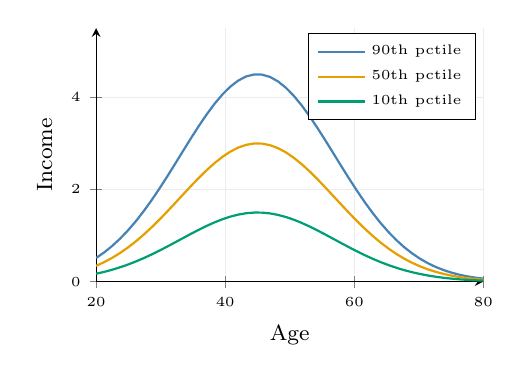
\begin{tikzpicture}
\begin{axis}[
    width=6.5cm, height=4.8cm,
    xlabel={Age}, ylabel={Income},
    xlabel style={font=\footnotesize},
    ylabel style={font=\footnotesize},
    tick label style={font=\tiny},
    xmin=20, xmax=80, ymin=0, ymax=5.5,
    grid=major, grid style={gray!15},
    legend style={font=\tiny, at={(0.98,0.98)}, anchor=north east},
    axis lines=left,
]
    \addplot[thick, softblue, domain=20:80, samples=50]
        {4.5*exp(-0.5*((x-45)/12)^2)};
    \addlegendentry{90th pctile}
    \addplot[thick, softorange, domain=20:80, samples=50]
        {3.0*exp(-0.5*((x-45)/12)^2)};
    \addlegendentry{50th pctile}
    \addplot[thick, softgreen, domain=20:80, samples=50]
        {1.5*exp(-0.5*((x-45)/12)^2)};
    \addlegendentry{10th pctile}
\end{axis}
\end{tikzpicture}\\
{\tiny Stylized income-by-age profiles}
\end{center}
\end{columns}
\end{frame}

% --- Slide 6: Dynamic Stochastic Models ---
\begin{frame}{Dynamic Stochastic General Equilibrium Models}
\textbf{Generic formulation:} find policy functions $p(\cdot)$ such that
\[
\E{G\bigl(\x_t,\,\x_{t+1},\,p(\x_t),\,p(\x_{t+1})\bigr) \;\Big|\; \x_t,\,p(\x_t)} = 0
\]
with transition law $\x_{t+1} = h\bigl(\x_t,\,p(\x_t),\,\varepsilon_{t+1}\bigr)$.

\vspace{0.4em}
\textbf{Four computational challenges} (Azinovic, Gaegauf \& Scheidegger, 2022):
\begin{enumerate}
    \setlength{\itemsep}{1pt}
    \item \emphc{Stochasticity}: nontrivial expectations over $\varepsilon_{t+1}$ and the ergodic distribution
    \item \emphc{High-dimensional} state space: heterogeneity, many assets, many shocks all push $d$ up
    \item \emphc{Strong nonlinearities / kinks} from occasionally binding constraints and regime switches
    \item \emphc{Irregular geometry} of the ergodic set: recurrent states are not a hypercube
\end{enumerate}

\vspace{0.2em}
{\footnotesize No classical method addresses all four jointly: sparse grids cover (1-3) but fail past $d \sim 20$; Gaussian processes cover (1,2,4) but choke on large data.}
\end{frame}

% --- Slide 7: What is High-Dimensional? ---
\begin{frame}{What is High-Dimensional?}
\begin{center}
\begin{tabular}{rrl}
\toprule
\textbf{Dimensions $d$} & \textbf{Grid points $n^d$} & \textbf{Runtime} \\
\midrule
1 & $10$ & 10 seconds \\
2 & $100$ & 2 minutes \\
5 & $10^5$ & 1 day \\
10 & $10^{10}$ & 317 years \\
20 & $10^{20}$ & $\sim 3$ trillion years \\
\bottomrule
\end{tabular}
\end{center}

\vspace{0.5em}
{\small Assumes $n = 10$ grid points per dimension and 1 second per evaluation.}

\vspace{0.5em}
\textbf{Three remedies:}
\begin{enumerate}
    \item \emphc{Sparse grids}~(Brumm \& Scheidegger, 2017)
    \item \emphc{Random grids}~(Rust, 1997)
    \item \emphc{Neural networks}~(this lecture)
\end{enumerate}
\end{frame}

% --- Slide 8: Volumes in High Dimensions ---
\begin{frame}{Volumes in High Dimensions}
\begin{center}
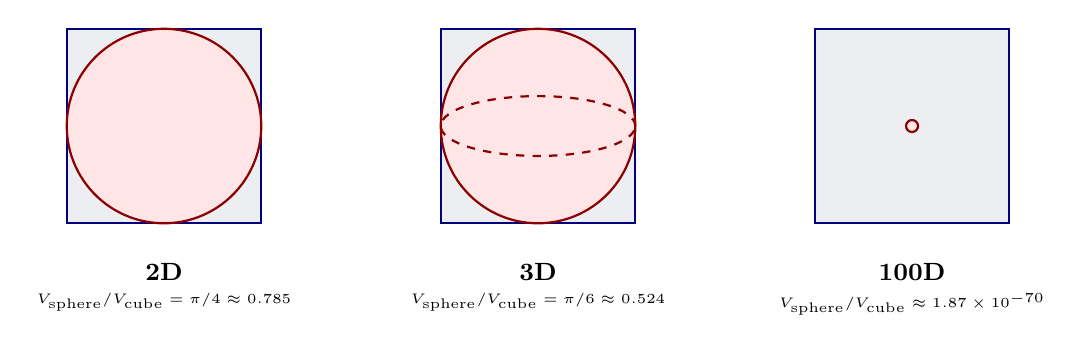
\begin{tikzpicture}[scale=0.95]
% 2D
\begin{scope}[shift={(0,0)}]
    \draw[thick, uzhblue, fill=uzhgreylight] (-1.3,-1.3) rectangle (1.3,1.3);
    \draw[thick, darkred, fill=red!10] (0,0) circle (1.3);
    \node[below, font=\small\bfseries] at (0,-1.7) {2D};
    \node[below, font=\tiny] at (0,-2.1) {$V_{\text{sphere}}/V_{\text{cube}} = \pi/4 \approx 0.785$};
\end{scope}
% 3D
\begin{scope}[shift={(5,0)}]
    \draw[thick, uzhblue, fill=uzhgreylight] (-1.3,-1.3) rectangle (1.3,1.3);
    \draw[thick, darkred, fill=red!10] (0,0) circle (1.3);
    \draw[thick, darkred, dashed] (0,0) ellipse (1.3 and 0.4);
    \node[below, font=\small\bfseries] at (0,-1.7) {3D};
    \node[below, font=\tiny] at (0,-2.1) {$V_{\text{sphere}}/V_{\text{cube}} = \pi/6 \approx 0.524$};
\end{scope}
% 100D
\begin{scope}[shift={(10,0)}]
    \draw[thick, uzhblue, fill=uzhgreylight] (-1.3,-1.3) rectangle (1.3,1.3);
    \draw[thick, darkred, fill=red!10] (0,0) circle (0.08);
    \node[below, font=\small\bfseries] at (0,-1.7) {100D};
    \node[below, font=\tiny] at (0,-2.1) {$V_{\text{sphere}}/V_{\text{cube}} \approx 1.87 \times 10^{-70}$};
\end{scope}
\end{tikzpicture}
\end{center}

\vspace{0.4em}
\begin{block}{Implication}
In high dimensions, \emphc{almost all volume is in the corners}. Grid-based methods waste most of their evaluation points in regions that barely contribute to the integral or approximation.
\end{block}
\end{frame}

% --- Slide 9: Nonlinearities and Kinks ---
\begin{frame}{Nonlinearities and Kinks}
\begin{columns}[T]
\column{0.52\textwidth}
\textbf{Where do kinks come from?}
\begin{itemize}
    \setlength{\itemsep}{1pt}
    \item \emphc{Borrowing constraints}: $a_{t+1}\ge \underline{a}$
    \item \emphc{Zero lower bound}: $i_t \ge 0$
    \item \emphc{Short-sale / participation}: corner solutions
    \item \emphc{Default, regime switches, indivisibilities}
\end{itemize}

\vspace{0.4em}
Occasionally binding constraints $\Rightarrow$ policy functions are \emphc{non-smooth} at the boundary of the binding region.

\vspace{0.4em}
{\footnotesize Polynomial / spectral methods lose accuracy; sparse grids can resolve kinks but only for $d\lesssim 20$. Neural networks handle kinks natively via ReLU-type activations.}

\column{0.48\textwidth}
\begin{center}
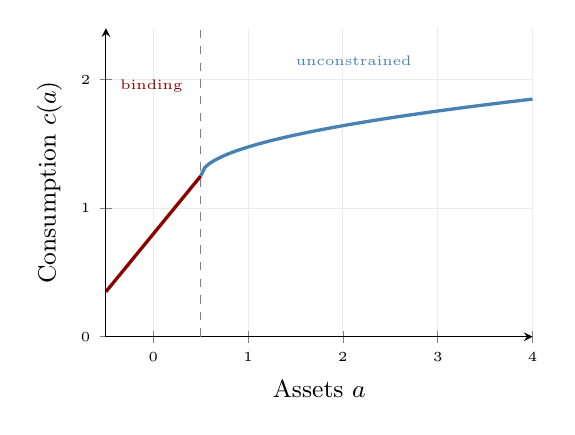
\begin{tikzpicture}
\begin{axis}[
    width=7cm, height=5.5cm,
    xlabel={Assets $a$}, ylabel={Consumption $c(a)$},
    xlabel style={font=\small},
    ylabel style={font=\small},
    tick label style={font=\tiny},
    xmin=-0.5, xmax=4, ymin=0, ymax=2.4,
    grid=major, grid style={gray!15},
    axis lines=left,
    samples=80,
]
    \addplot[very thick, darkred, domain=-0.5:0.5] {0.35 + 0.90*(x+0.5)};
    \addplot[very thick, softblue, domain=0.5:4] {1.25 + 0.32*sqrt(x-0.5)};
    \draw[dashed, gray] (axis cs:0.5,0) -- (axis cs:0.5,2.4);
    \node[font=\tiny, anchor=north] at (axis cs:0.5,0) {$a=\underline{a}$};
    \node[font=\tiny, darkred, anchor=west] at (axis cs:-0.45,1.95) {binding};
    \node[font=\tiny, softblue, anchor=west] at (axis cs:1.4,2.15) {unconstrained};
\end{axis}
\end{tikzpicture}\\
{\tiny Kinked consumption policy at the borrowing limit}
\end{center}
\end{columns}
\end{frame}

% --- Slide 10: The Ergodic Set is not a Hypercube ---
\begin{frame}{The Ergodic Set Is Not a Hypercube}
\small
\textbf{Grid-based} methods tile the full hypercube $\x \in [\x_{\min}, \x_{\max}]^d$.  \textbf{But} simulated states drawn from the model's law of motion fill only a \emphc{thin, irregular} subset, the \emphc{ergodic set} (states actually visited by the economy), often $\ll 1\%$ of the hypercube {\footnotesize (Judd, Maliar \& Maliar, 2011)}.

\vspace{0.3em}
\begin{center}
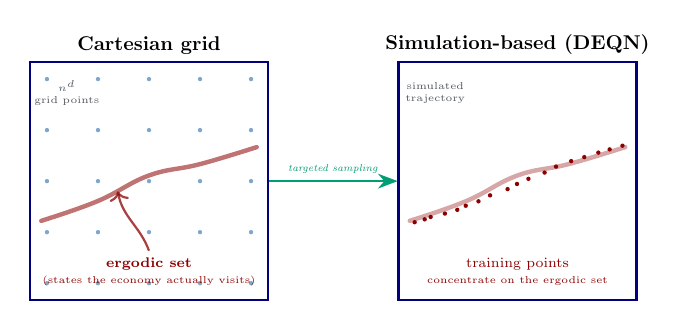
\begin{tikzpicture}[scale=0.72, transform shape,
    dotblue/.style={circle, fill=softblue!70, inner sep=0pt, minimum size=2.2pt},
    dotred/.style={circle, fill=darkred,      inner sep=0pt, minimum size=2.2pt},
    cube/.style={rectangle, draw=uzhblue, thick, minimum width=4.2cm, minimum height=4.2cm}]
    % Left panel: Cartesian grid
    \node[cube, label={above:\textbf{Cartesian grid}}] (g) at (0,0) {};
    \foreach \i in {-1.8,-0.9,0,0.9,1.8} {
        \foreach \j in {-1.8,-0.9,0,0.9,1.8} {
            \node[dotblue] at (\i,\j) {};
        }
    }
    \draw[darkred, ultra thick, opacity=0.55, line cap=round]
        plot[smooth, tension=0.7] coordinates {(-1.9,-0.7) (-0.9,-0.35) (0,0.1) (0.9,0.3) (1.9,0.6)};
    \node[font=\scriptsize, text=darkred, align=center] (ergL) at (0,-1.6)
        {\textbf{ergodic set}\\{\tiny (states the economy actually visits)}};
    \draw[->, darkred, thick, opacity=0.75]
        (ergL.north) to[out=110,in=-80,looseness=1.0] (-0.55,-0.18);
    \node[font=\tiny, text=uzhgreydark, align=center] at (-1.45,1.55) {$n^d$\\grid points};

    % Right panel: Simulation-based
    \node[cube, label={above:\textbf{Simulation-based (DEQN)}}] (s) at (6.5,0) {};
    \begin{scope}[xshift=6.5cm]
        \draw[darkred, ultra thick, opacity=0.35, line cap=round]
            plot[smooth, tension=0.7] coordinates {(-1.9,-0.7) (-0.9,-0.35) (0,0.1) (0.9,0.3) (1.9,0.6)};
        \foreach \t in {-1.85,-1.65,-1.5,-1.3,-1.1,-0.9,-0.7,-0.45,-0.2,0,0.2,0.45,0.7,0.95,1.15,1.4,1.6,1.85}{
            \pgfmathsetmacro{\yy}{-0.7 + 1.3*(\t + 1.9)/3.8 + 0.08*sin(deg(\t*1.4))}
            \pgfmathsetmacro{\xx}{\t + 0.04*rand}
            \node[dotred] at (\xx,\yy) {};
        }
        \node[font=\tiny, text=uzhgreydark, align=center] at (-1.45,1.55)
            {simulated\\trajectory};
        \node[font=\scriptsize, text=darkred, align=center] at (0,-1.6)
            {training points\\{\tiny concentrate on the ergodic set}};
    \end{scope}

    \draw[-{Stealth[length=2.5mm]}, thick, softgreen]
        (g.east) -- node[above, font=\tiny, text=softgreen]{\textit{targeted sampling}} (s.west);
\end{tikzpicture}
\end{center}

\vspace{-0.3em}
\begin{center}
{\footnotesize A full Cartesian grid \emphc{wastes} most of its work in regions the economy never visits $\Rightarrow$ motivates \emphc{simulation-based, grid-free} methods.}
\end{center}
\end{frame}

% --- Slide 11: Abstract Problem Formulation ---
\begin{frame}{Abstract Problem Formulation}
We need a numerical method that satisfies:

\vspace{0.4em}
\begin{enumerate}
    \item \textbf{Global approximation:} avoid purely local perturbation solutions
    \item \textbf{Approximate solutions:} accept small residual error $\varepsilon > 0$
    \item \textbf{Grid-free in practice:} avoid explicit tensor-product growth $n^d$
    \item \textbf{Flexible geometry:} handle nonlinearities, kinks, and irregular ergodic sets
    \item \textbf{Parallel-friendly:} benefit from \emphc{parallelization} on modern hardware
\end{enumerate}

\vspace{0.6em}
\begin{center}
$\Rightarrow$ \textbf{DEQNs address this wishlist well in practice,}
while \emphc{mitigating} rather than eliminating high-dimensional costs.
\end{center}
\end{frame}

% --- Slide 10: Our Solution: DEQNs ---
\begin{frame}{Our Solution: Deep Equilibrium Nets}
\textbf{Core idea} (Azinovic, Gaegauf \& Scheidegger, 2022):

\vspace{0.3em}
Replace the traditional grid-based solution with a \emphc{neural network} trained to satisfy economic equilibrium conditions.

\vspace{0.5em}
\begin{block}{Three Key Ingredients}
\begin{enumerate}
    \item \textbf{Equilibrium error as loss function:} use the economic equations $G(\cdot) = 0$ directly, with \emphc{no labeled data} needed
    \item \textbf{Stochastic gradient descent:} optimize network parameters $\rho$ via SGD on mini-batches
    \item \textbf{Simulated paths:} draw training points from the \emphc{ergodic distribution} of the model itself
\end{enumerate}
\end{block}

\vspace{0.3em}
{\small $\Rightarrow$ This turns \emphc{solving} an economic model into \emphc{training} a neural network.}
\\[2pt]
{\scriptsize It avoids explicit state-space grids, but expectation accuracy, sampling quality, and optimization still matter.}
\end{frame}

% ============================================================================
% PART II: FROM ANNs TO DEQNs
% ============================================================================

% --- Slide 11: Section Divider ---
\begin{frame}{}
\vfill
\begin{center}
{\Huge \textcolor{uzhblue}{\textbf{Part II}}}\\[12pt]
{\LARGE From ANNs to Deep Equilibrium Nets}
\end{center}
\vfill
\end{frame}

\end{document}
